\section{Costo previsto del sistema}
Sebbene lo scopo di questa tesi sia di evidenziare 
l'effetto delle scelte implementative sulla scalabilità del sistema,
l'aspetto economico non può essere ignorato durante la realizzazione di un progetto.
Si cerca quindi di prevedere la spesa effettiva delle risorse utilizzate in base a un utilizzo possibile,
soffermandosi maggiormente sulla dinamica di definizione dei parametri richiesti 
rispetto all'effettiva necessità, 
che può variare in base al mercato dell'applicazione o alla sua maturità.\\
\\
Essendo l'applicazione in fase prototipale, 
si può solamente provare a dedurre l'effettivo utilizzo delle risorse proporzionalmente al carico previsto.
Per il calcolo del costo del sistema si è deciso di considerare un carico 
di cinquemila utenti attivi giornalmente, 
che indica un utilizzo consistente e maturo dell'applicazione.\\
\\
Per stimare il costo del sistema viene usato uno strumento offerto da Azure chiamato Pricing Simulator.
Questo strumento, accessibile online, 
permette di calcolare il costo dell'utilizzo delle risorse in base all'utilizzo che si prevede di farne.
Per ogni servizio, in base alle sue peculiarità, 
viene chiesto l'inserimento di dati specifici per il suo utilizzo.
Per alcuni servizi, in cui era stato adottato il piano di utilizzo più economico, 
è stato necessario assumere l'adozione di un piano 
che permetta effettivamente di gestire il carico previsto.
I costi vengono calcolati mensilmente.\\
\\
Azure Static Web App prevede due tipologie di piani, gratuito o standard.
Il piano gratuito fornisce 100 gigabyte di bandwidth e 
un massimo di 0.5 gigabyte di memoria.
La dimensione attuale dell'applicazione risulta di circa 20 megabyte,
che viene però compressa dal sistema.
Il limite della memoria non risulta quindi un problema,
ma bisogna verificare che non si superi la quantità fornita di bandwidth.\\
\\
La dimensione dei dati ricevuti dal browser in fase di caricamento del sito 
ammonta a un massimo di 10 megabyte.
Questa quantità si riduce notevolmente se il sito è già stato caricato in cache, 
a un massimo stimato di 250 kilobyte.
Considerando che il metodo di fruizione principale del progetto avvenga tramite applicazione,
si stimano 2500 utenti mensili da browser.
Stimando un utilizzo quotidiano dell'applicazione, 
il primo giorno sarà necessario scaricare l'intero sito, 
mentre le volte successive solo aggiornare la cache, 
che porta il calcolo della quantità di dati effettivamente trasferita al seguente:\\
2500 x (10 Mb + 250 Kb x 29) = 43 Gb.\\
I quarantatrè gigabyte così previsti rientrano ampiamente nei cento offerti,
permettendo l'utilizzo del piano gratuito.\\
\\
Per stimare il costo delle Azure Functions è necessario calcolare
le interazioni totali mensili con gli utenti.
Queste vengono previste per 200 richieste giornaliere,
che includono sia richieste in scrittura che in lettura.
Si calcolano così un milione di invocazioni giornaliere, 
per un totale di trenta milioni di chiamate mensili.\\
\\
Dai test si evince una durata media delle funzioni che si aggira sui 200 millisecondi.
Per stare sul sicuro, la durata prevista per richiesta 
viene arrotondata a 250 millisecondi.
Allo stesso modo, si prevede un utilizzo medio di 0.5 gigabyte di memoria per ogni invocazione.
Nel calcolo bisogna considerare le risorse gratuite e
un costo di €0.000015 per GB/s e €0.117 per milione di richieste,
portando la spesa totale prevista attorno ai € 60.\\
\begin{figure}[htbp]
    \begin{center}
        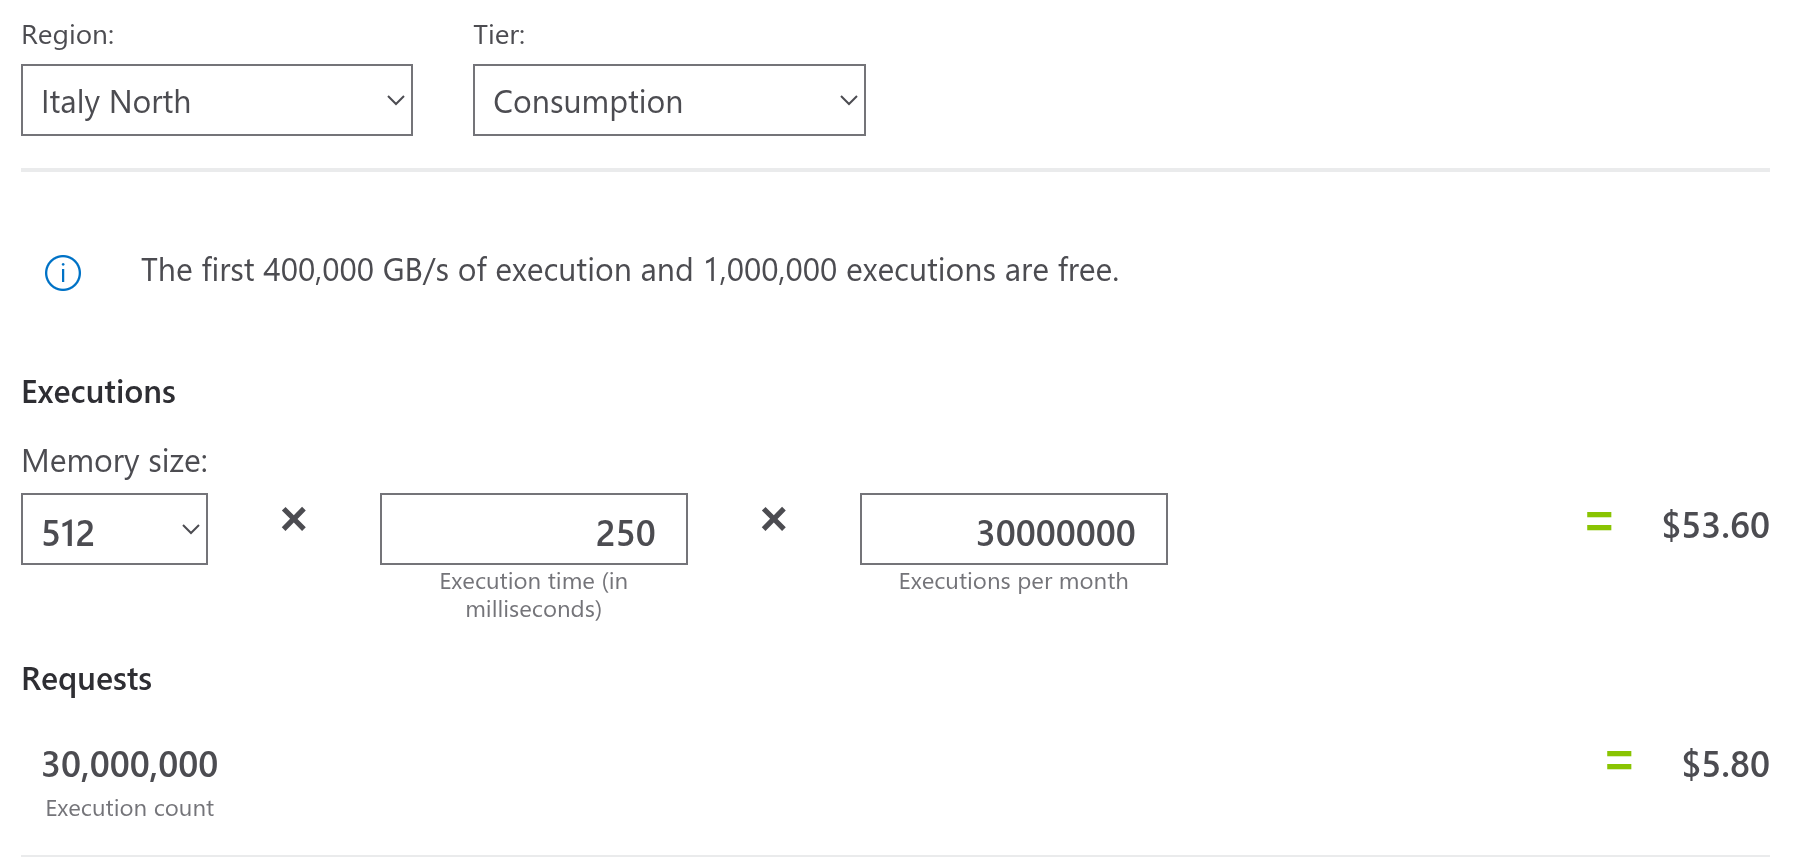
\includegraphics[width=\textwidth]{pricing_functions.png}
        \caption{Calcolo per il costo delle Azure Functions}
    \end{center}
\end{figure}
\\
Il costo del database, implementato con Azure Cosmos DB, 
varia in base alle Request Units al secondo(RU/s) usate.
Ogni richiesta consuma una certa quantità di RU, 
in base al carico computazionale necessario.
Bisogna quindi stimare le richieste al secondo,
e il loro consumo di Request Unit.
Considerando che la quasi totalità delle richieste 
verso le Azure Functions implicano un accesso al database,
le invocazioni per secondo possono essere calcolate 
dividendo le richieste giornaliere per i secondi di una giornata,
facendo così risultare una media di 12 richieste al secondo.\\
\begin{figure}[htbp]
    \begin{center}
        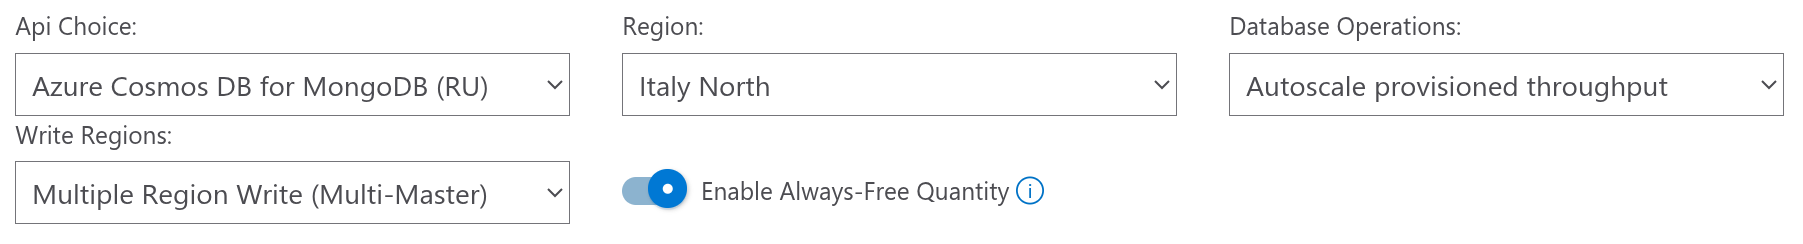
\includegraphics[width=\textwidth]{pricing_settings_cosmos.png}
        \caption{Impostazioni del server Cosmos}
    \end{center}
\end{figure}
\\
Il consumo medio di RU registrato durante i test 
varia tra i 10 e i 20 RU per richiesta.
Per sicurezza, si considera il consumo medio di un'operazione sul database
di 30 RU.
Risulta così una media di 360 RU/s,
che non fornisce però informazioni sul picco del carico. 
Utilizzando un piano di tipologia autoscale,
che modifica in automatico le risorse del database in base al carico effettivo,
bisogna stabilire il carico massimo che si prevede il database debba sostenere,
tenendo però presente che la quantità minima di risorse sempre stanziate sarà del suo 10\%.\\
\\
Non essendo in possesso di dati relativi all'effettivo utilizzo dell'applicazione,
Stimiamo un utilizzo massimo pari a 5 volte quello previsto, 
pari a 60 richieste al secondo.
Questo porta a un massimo di 1800 RU/s, con una media prevista del 20\%.
Sottraendo i primi 1000 RU/s e moltiplicando i restanti per il costo orario di € 0.016, 
il costo totale previsto per l'utilizzo di Azure Cosmos si aggira intorno ai € 20.\\
\begin{figure}[htbp]
    \begin{center}
        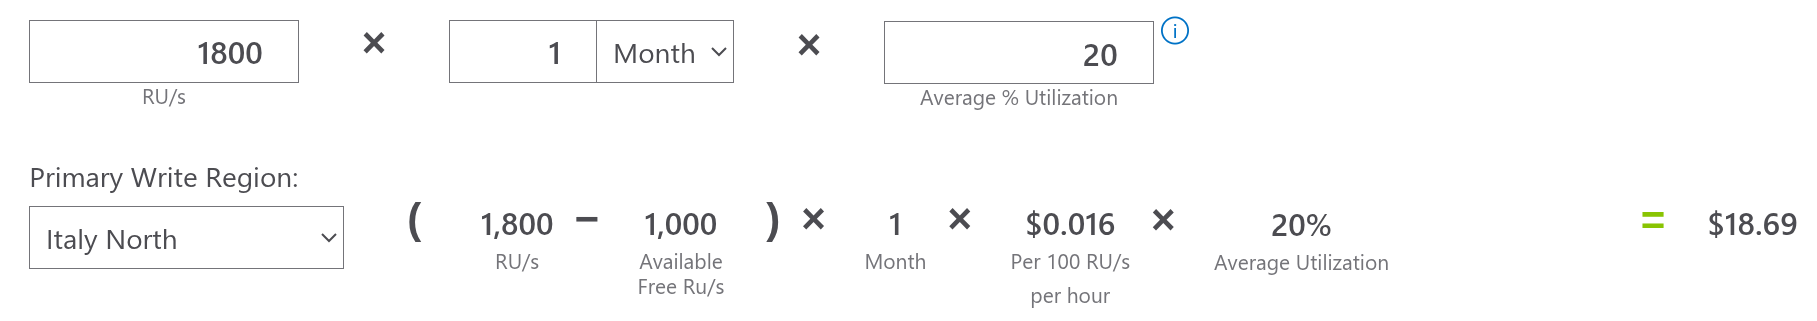
\includegraphics[width=\textwidth]{pricing_cosmos.png}
        \caption{Calcolo per il costo di Cosmos}
    \end{center}
\end{figure}
\clearpage






Key vault
1 richiesta ogni 10 operazioni
\\



storage container
30 immagini al giorno, 5000 * 4mb = 600 gb
necessario comprimere l'immagine a 200 kb

PubSub
 1 utenza, 
 messaggi da 1kb, si considerano metà delle richieste come richieste in scrittura, 
 ma vengono inviati solo agli utenti presenti
 e quindi 15.000.000 * 1Kb * 10 canali broadcast = 30 GB.

Authentication
Gratis per i primi 50000 di utenti attivi mensilie.

Queue
al mese 30.000.000 operazioni di lettura
30.000.000 opeazioni di scrittura.

capacità totale di 50 Gb, sufficienti perché, 
una volta letto il messaggio, questo viene rimosso dalla coda.

servicebus
-confirm/update event 300.000 giornaliere = 9 milioni mensili



Virtual network 
free of charge

riconsiderare PubSub. 
compressione immagini.
totale.

\clearpage
\chapter*{Conclusioni}
\addcontentsline{toc}{chapter}{Conclusione}

\begin{figure}[htbp]
    \begin{center}
        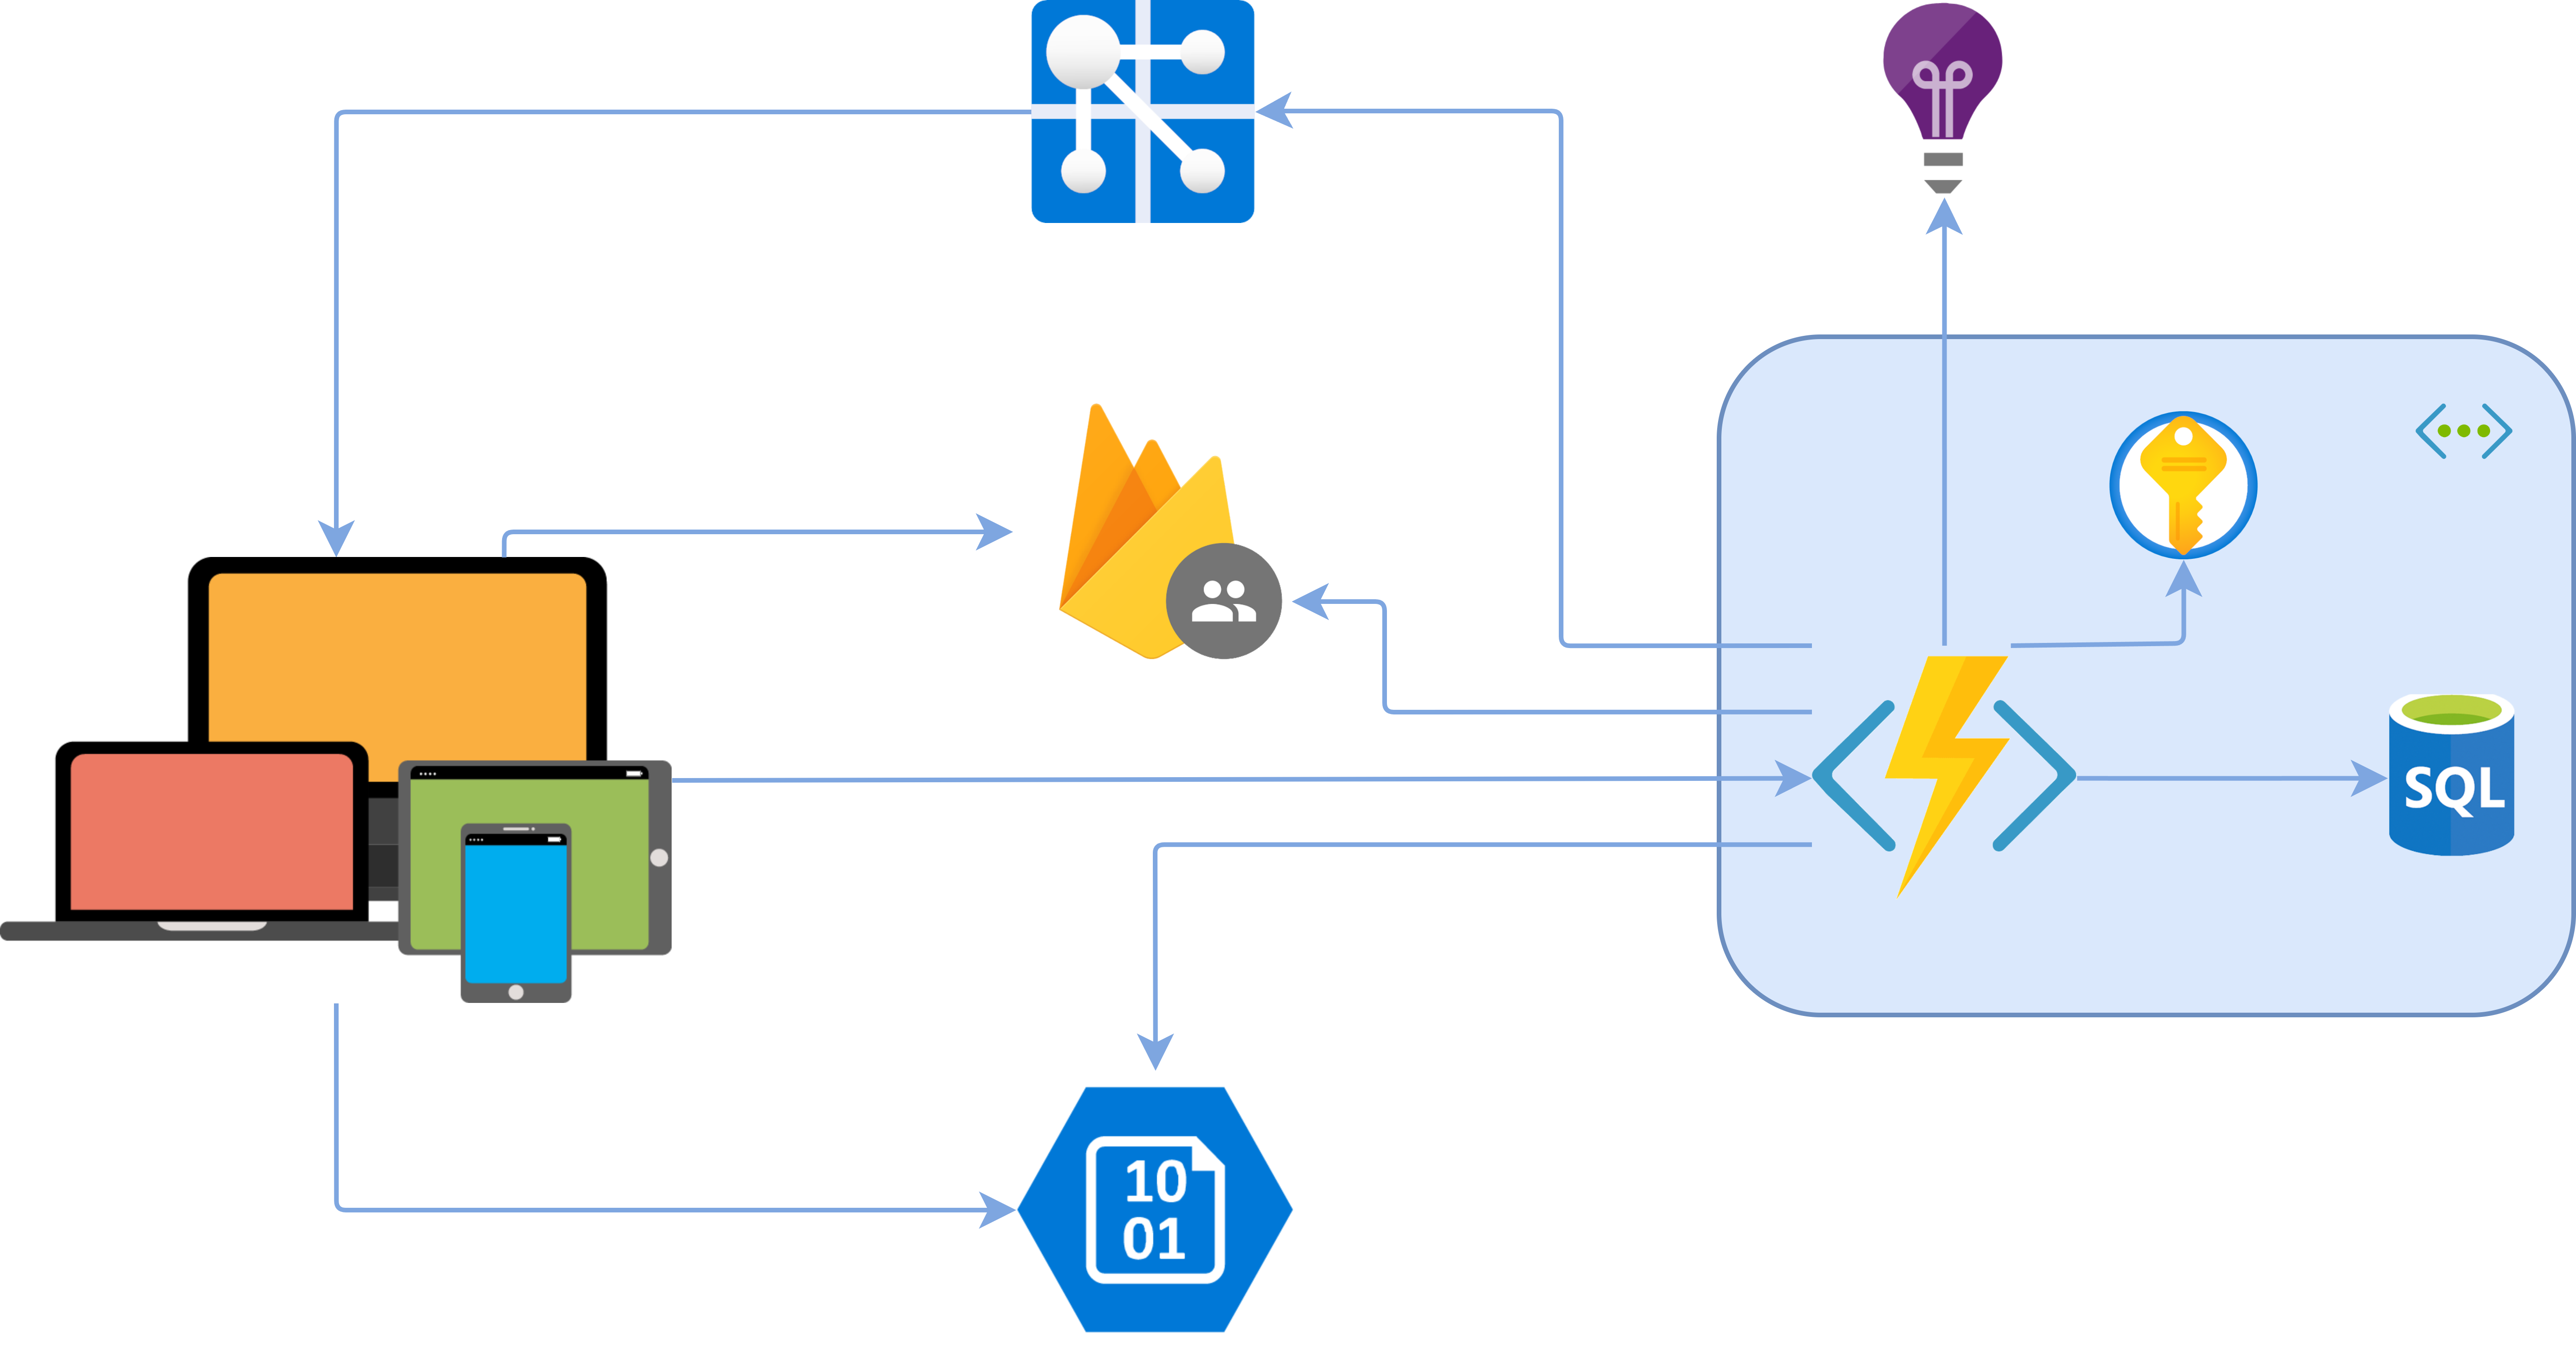
\includegraphics[width=\textwidth]{ImplementazioneArchitettura.png}
        \caption{Grafico dell'architettura di WYD}
    \end{center}
\end{figure}
\clearpage

\section{Sviluppi futuri}
Gli sviluppi futuri potranno comprendere, in base a decisioni di marketing:
\begin{itemize}
    \item La visualizzazione degli impegni degli altri profili
    \item L'implementazione di una chat per ogni gruppo
    \item Sviluppo di strumenti utili all'organizzazione dei gruppi, quali:
          \begin{itemize}
              \item form per combinare le disponibilità reciproche
              \item appunti condivisi(liste della spesa o note su chi porta cosa)
              \item calcolo delle spese compiute da ciascun componente
          \end{itemize}
    \item La creazione di profili pubblici che possono essere seguiti
    \item La creazione di eventi pubblici
    \item Una funzionalità di ricerca degli eventi o dei profili pubblici
    \item Supporto alla gestione di prenotazione e organizzazione degli eventi, dalle liste di attesa alla vendita dei biglietti
    \item La possibilità per le aziende di gestire in locale il proprio server e i relativi dati
\end{itemize}
\clearpage

\chapter*{Fonti bibliografiche e sitografia}
\addcontentsline{toc}{chapter}{Fonti bibliografiche e sitografia}

Object Management Group, OMG Unified Modelling Language Version 2.5.1, December 2017, https://www.omg.org/spec/UML/2.5.1/PDF

https://learn.microsoft.com/en-us/azure/reliability/reliability-cosmos-db-nosql
https://learn.microsoft.com/en-gb/azure/cosmos-db/throughput-serverless
https://learn.microsoft.com/en-gb/azure/cosmos-db/provision-throughput-autoscale